\section{Results}

\subsection{Models Performance}

We were unable to create embeddings for every single protein in our holdout test sets. Therefore, to get comparable results between the baseline and enhanced models, we had no choice but to remove those entries, marginally decreasing the size of our sets from 816 DTIs for the classification models to 740 and from 102 DTIs for the regression models to 95.

\subsubsection{Classification Models}

Tables \ref{tbl:baseline_classification} and \ref{tbl:enhanced_classification} showcase the predictive performance of our baseline and enhanced classification models and as we can clearly see our embeddings did not have much of an impact, except possibly in the cases of the logistic regression where they seem to have negatively impacted it and the random forest classifier where they seem to have slightly improved performance as we can see from their metrics, and particularly the MCC score.

Our best models in both cases seem to be the K-nearest neighbour and random forest classifier, although all models, except the dummy ones obviously and the decision tree classifier, achieve close enough performances.

\subsubsection{Regression Models}
\label{subsubsec:Regression_Performance}

Tables \ref{tbl:baseline_regression} and \ref{tbl:enhanced_regression} showcase the predictive performance of our baseline and enhanced regression models and it could be argued that our embeddings in this case had a much more evident effect, positive in most cases, except obviously in the case of the linear regression model. However, given that the intervals are so spread out a decisive conclusion cannot be confidently reached.

In the case of the enhanced models, our best models seem to be the K-nearest neighbour regressor and the neural network. As for the case of the baseline models given that all our models achieve a negative R2 score, meaning worse than random, evidenced by achieving worse scores than the dummy regressor, we feel that it would be pointless to point out any of them.

There seem to be some promising results for the regression models and it would be interesting to see what performances they could achieve with a more extensive and diverse dataset than the one we used.

\subsubsection{Model Bias}

All classification models, regardless of type, seem to have particular difficulty in recognising the negative class, meaning an inactive DTI, with actually the number of False Positives surpassing True Negatives in most cases which could be in part explained by the class imbalance present in our dataset. We expect that actively tackling this problem in future work will lead to a noticeable improvement in the predictive performance of the models.

\subsection{Important Descriptors}

As we have previously discussed in Subsection \ref{subsubsec:Feature_Selection}, RFECV was used to find the most important drug and protein sequence descriptors. The intersection between the descriptors found to be important for both classification and regression includes the drug descriptors showcased in Table \ref{tbl:important_drug_descriptors} and the protein sequence descriptors showcased in Table \ref{tbl:important_protein_sequence_descriptors}.

\bigskip
\bigskip

\subsection{Embeddings}

We were able to produce 11,034 protein structural embeddings with 256 dimensions placed into a dictionary which was then pickled for easy storage and retrieval. To visualise them we used PCA to project them into a two-dimensional space and plotted them. 

Looking at Figure \ref{fig:Embeddings_PCA} we can see that most of the embeddings are closely packed together with a few noticeable outliers. However, given the ineffectiveness of our embeddings we cannot draw any conclusions from their spread.

\subsubsection{Performance}

Given that our enhanced machine-learning models, which utilised the embeddings from our transfer learning process, and the neural networks which calculated the protein structural representations optimised specifically for DTI prediction achieved similar performance to that of the baseline models it most certainly appears that we have not efficiently encoded the structural information of proteins.

Considering that we used a very similar deep learning architecture to process the protein contact maps with the successful study conducted by \citet{Jiang2020} we speculate that our choice of 10 \AA {} instead of the 8 \AA {} used by the study mentioned above may have played a significant role in our embeddings ineffectiveness. However, without any further experimentation this remains an unproven theory.

It is also possible that the process used is better suited for predicting the binding affinity of DTIs, given the promising results of Subsection \ref{subsubsec:Regression_Performance}, instead of their binary relationship which may require a more complex representation and processing of protein structures. Such approaches include the studies of \citet{Sofia} and \citet{Lee2022} where they chose a more targeted strategy using each protein's binding pockets instead of its whole structure.

\begin{figure}[!hb]
    \centering
    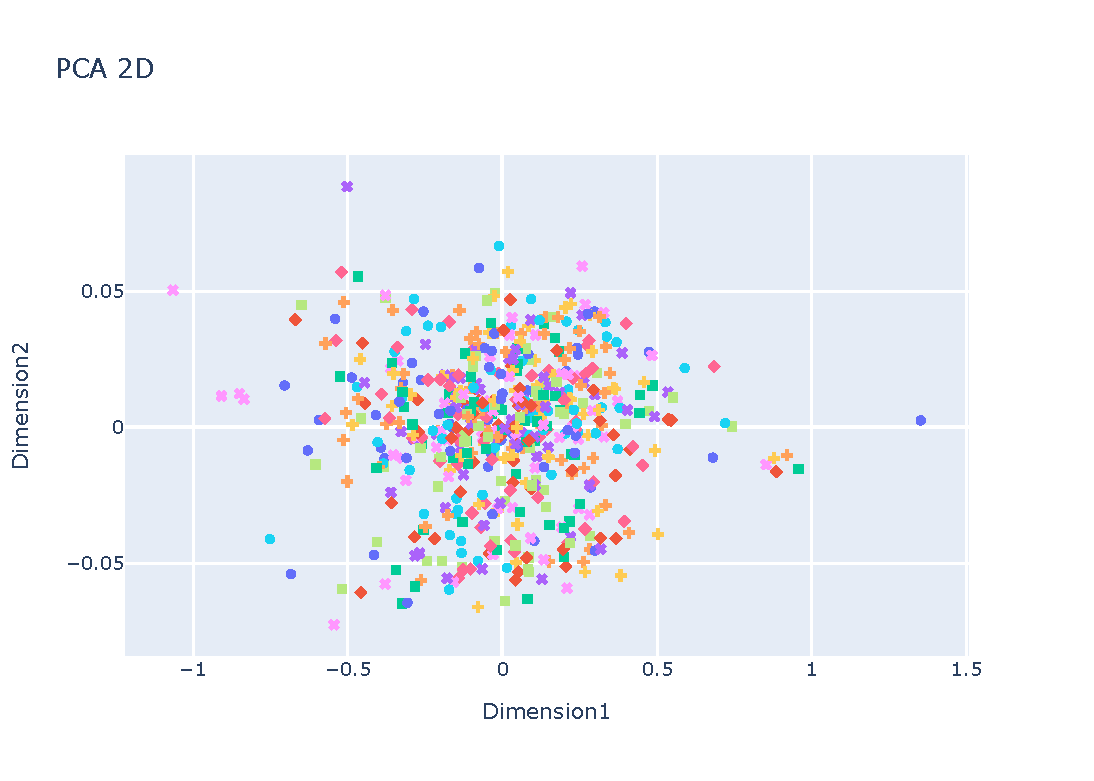
\includegraphics[width=1.0\linewidth]{images/Embeddings_PCA.pdf}    
    \caption{PCA plot of our created protein structural embeddings after projecting them to a two-dimensional space. *Each scatter point is a unique embedding regardless of shape and colour.}
    \label{fig:Embeddings_PCA} 
\end{figure}

\bigskip
\bigskip
\bigskip
\bigskip
\bigskip
\bigskip


\begin{table*}
    \tabcolsep=0.08cm
    \begin{tabular}{llllll}
    \toprule
                                     Model &        Accuracy  &           Recall &        Precision &               F1 & MCC \\
    \midrule
                          Dummy Classifier & 0.68 (0.64-0.72) & 1.00 (1.00-1.00) & 0.68 (0.64-0.72) & 0.81 (0.78-0.84) &                          0 (0-0) \\
                       Logistic Regression & 0.73 (0.69-0.77) & 0.86 (0.83-0.90) & 0.77 (0.73-0.81) & 0.81 (0.78-0.84) &                  0.34(0.24-0.43) \\
      Linear Support Vector Classification & 0.73 (0.69-0.77) & 0.87 (0.84-0.91) & 0.77 (0.72-0.81) & 0.82 (0.78-0.85) &                 0.34 (0.25-0.43) \\
            K-Nearest Neighbour Classifier & 0.75 (0.71-0.79) & 0.83 (0.79-0.87) & 0.81 (0.77-0.85) & 0.82 (0.79-0.85) &                 0.42 (0.33-0.51) \\
                  Decision Tree Classifier & 0.64 (0.60-0.68) & 0.71 (0.66-0.76) & 0.75 (0.70-0.79) & 0.73 (0.69-0.76) &                 0.19 (0.10-0.28) \\
                  Random Forest Classifier & 0.75 (0.71-0.79) & 0.93 (0.90-0.96) & 0.76 (0.72-0.79) & 0.84 (0.81-0.86) &                 0.37 (0.28-0.45) \\
    Stochastic Gradient Descent Classifier & 0.73 (0.69-0.77) & 0.86 (0.83-0.90) & 0.77 (0.73-0.81) & 0.81 (0.78-0.84) &                 0.33 (0.25-0.42) \\
    \bottomrule
    \end{tabular}
    \caption{Testing set (740 DTIs) performance of baseline classification models}
    \label{tbl:baseline_classification}
\end{table*}


\begin{table*}
    \tabcolsep=0.08cm
    \begin{tabular}{llllll}
    \toprule
                                     Model &        Accuracy  &           Recall &        Precision &               F1 &              MCC \\
    \midrule
                          Dummy Classifier & 0.68 (0.64-0.73) & 1.00 (1.00-1.00) & 0.68 (0.64-0.73) & 0.81 (0.78-0.84) &          0 (0-0) \\
                       Logistic Regression & 0.72 (0.68-0.76) & 0.92 (0.89-0.95) & 0.73 (0.69-0.78) & 0.82 (0.79-0.84) & 0.28 (0.18-0.37) \\
      Linear Support Vector Classification & 0.72 (0.68-0.76) & 0.85 (0.81-0.89) & 0.77 (0.73-0.81) & 0.80 (0.77-0.84) & 0.32 (0.22-0.41) \\
            K-Nearest Neighbour Classifier & 0.75 (0.71-0.79) & 0.86 (0.82-0.90) & 0.79 (0.75-0.83) & 0.82 (0.79-0.85) & 0.40 (0.31-0.48) \\
                  Decision Tree Classifier & 0.62 (0.58-0.66) & 0.69 (0.64-0.74) & 0.74 (0.69-0.79) & 0.71 (0.67-0.75) & 0.17 (0.07-0.26) \\
                  Random Forest Classifier & 0.76 (0.72-0.80) & 0.92 (0.89-0.95) & 0.77 (0.73-0.81) & 0.84 (0.81-0.87) & 0.41 (0.32-0.50) \\
    Stochastic Gradient Descent Classifier & 0.73 (0.69-0.77) & 0.92 (0.88-0.94) & 0.75 (0.70-0.79) & 0.82 (0.79-0.85) & 0.31 (0.22-0.40) \\
                            Neural Network &              0.7 &              0.7 &             0.83 &             0.79 &             0.36 \\
    \bottomrule
    \end{tabular}
    \caption{Testing set (740 DTIs) performance of enhanced classification models}
    \label{tbl:enhanced_classification}
\end{table*}

\begin{table*}
    \centering
    \begin{tabular}{lll}
    \toprule
                                    Model & Negated Mean Absolute Error &                     R2 \\
    \midrule
                          Dummy Regressor &      -1.96 (-2.32 to -1.65) &     -0.03 (-0.43 to 0) \\
                        Linear Regression &      -3.57 (-4.39 to -2.78) & -3.10 (-7.20 to -1.28) \\
         Linear Support Vector Regression &      -2.34 (-2.82 to -1.83) & -0.70 (-2.49 to -0.01) \\
            K-Nearest Neighbour Regressor &      -1.50 (-2.06 to -1.02) &  -0.17 (-0.60 to 0.22) \\
                  Decision Tree Regressor &      -3.10 (-3.93 to -2.33) & -2.44 (-7.14 to -0.92) \\
                  Random Forest Regressor &      -2.48 (-2.85 to -2.15) & -0.50 (-1.92 to -0.02) \\
    Stochastic Gradient Descent Regressor &      -2.40 (-3.05 to -1.87) & -0.97 (-2.96 to -0.10) \\
    \bottomrule
    \end{tabular}
    \caption{Testing set (95 DTIs) performance of baseline regression models.}
    \label{tbl:baseline_regression}
\end{table*}

\begin{table*}
    \centering
    \begin{tabular}{lll}
    \toprule
                                    Model &  Negated MAE &                               R2 \\
    \midrule
                          Dummy Regressor &       -1.95 (-2.30 to -1.66) &               -0.03 (-0.29 to 0) \\
                        Linear Regression & -130.78 (-157.40 to -105.42) & -5231.97 (-11775.09 to -2645.58) \\
         Linear Support Vector Regression &       -2.20 (-2.60 to -1.83) &            -0.34 (-1.44 to 0.05) \\
            K-Nearest Neighbour Regressor &       -1.36 (-1.89 to -0.92) &             0.01 (-0.20 to 0.33) \\
                  Decision Tree Regressor &       -2.77 (-3.65 to -1.93) &           -2.35 (-6.89 to -0.61) \\
                  Random Forest Regressor &       -2.43 (-2.82 to -2.10) &               -0.50 (-1.79 to 0) \\
    Stochastic Gradient Descent Regressor &       -1.75 (-2.18 to -1.34) &            -0.09 (-0.65 to 0.15) \\
                           Neural Network &                        -1.56 &                             0.09 \\
    \bottomrule
    \end{tabular}
    \caption{Testing set (95 DTIs) performance of enhanced regression models.}
    \label{tbl:enhanced_regression}
\end{table*}

\begin{table*}
    \centering
    \begin{tabular}{llll}
    \toprule
    MolecularWeight & XLogP & ExactMass & MonoisotopicMass \\
    TPSA & Complexity & HBondDonorCount & HBondAcceptorCount \\
    RotatableBondCount & HeavyAtomCount & AtomStereoCount & DefinedAtomStereoCount \\
    Volume3D & XStericQuadrupole3D & YStericQuadrupole3D & ZStericQuadrupole3D \\ FeatureCount3D &  FeatureAcceptorCount3D & FeatureDonorCount3D & FeatureCationCount3D \\ FeatureRingCount3D & FeatureHydrophobeCount3D & ConformerModelRMSD3D & EffectiveRotorCount3D \\
    ConformerCount3D & Fingerprint2D \\
    \bottomrule
    \end{tabular}
    \caption{Important drug descriptors for both classification and regression.}
    \label{tbl:important_drug_descriptors}
\end{table*}

\begin{table*}
    \centering
    \begin{tabular}{llll}
    \toprule
    CHOC760101.lag4.1 & hydrophobicity.Group3 & secondarystruct.Group1 & prop3.Tr1221 \\
    prop5.Tr1221 & VS562 & Schneider.Xr.N \\
    \bottomrule
    \end{tabular}
    \caption{Important protein sequence descriptors for both classification and regression.}
    \label{tbl:important_protein_sequence_descriptors}
\end{table*}

